\section{Publish/Subscribe}
Publish/Subscribe within DDS is split between the sending and the receiving part. This helps separate to the parts, since the receiver only needs to know what data is being communicated.

\subsection{Space, time, and flow decoupling}
When speaking about decoupling, either in space, time, or flow, it's a question about how coupled the producer and the consumer are in the different subjects.

\begin{description}
 \item[Space decoupling] \hfill \\
 Space refers to a situation, where the publisher and subscriber does not know each other.
 \item[Flow decoupling] \hfill \\
 If there is no flow blocking, speaking of data, by either the producer or the consumer, it is called flow decoupling.
 \item[Time decoupling] \hfill \\
 When the publisher and subscriber works asynchronous, they are decoupled in time.
\end{description}

\subsection{Middleware types and decoupling}
Different types of \emph{middlware} exists. \ref{DeInPa} shows a small part of the different types of \emph{middleware} that exists.
Below are explained, three different types, whether or not they decouple in space, time, or flow; \emph{RPC/RMI}, \emph{Notification(Observer D. Pattern)}, and \emph{Publish/Subscribe}.

\begin{figure}[ht!]
\centering
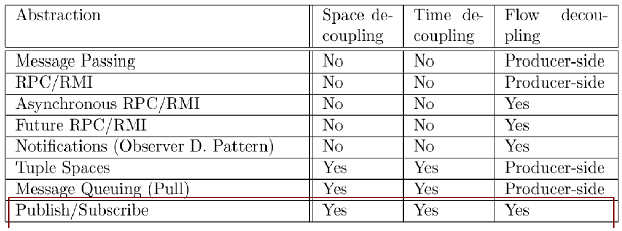
\includegraphics[width=150mm]{img/DecouplingInteractionParadigms.png}
\caption{Differences in \emph{middleware} types and decoupling - (from Many faces of public subscribe)}
\label{DeInPa}
\end{figure}

\begin{description}
\item[The publish/subscribe] type is a proven and reliable way of delivering information. It is decoupled in time, space, and flow - it works with space decoupling, since publisher and subscriber doesn't know each other. Time decoupling, because there are no rules about how the message shall live, and flow because there are no blocking of data. \\

\item[Notification(Observer D. Pattern)] is neither decoupled in space and time. It works by subscriber registers their interests directly with the publisher, so it's coupled in space. It works by two asynchronous invocations, but this is to obtain synchronous coupling - so it coupled in time. It is left to the publisher to manage communication, and therefore it is decoupled in flow.\\

\item[RPC(Remote Procedure Call)] is remote invocation used as distributions of interactions. This type is considered synchronous. It works by sending a asynchronous signal from the consumer, and the producer creates a response. This ensures a secure synchronous connection, and therefore the RPC is coupled in time, and also in space, since the an invoking object holds a reference to each of its invokers. There are created types, where it is created asynchronous, but this is less reliable.\\

\end{description}

\subsection{Topic, Content and Type based Publish/Subscribe}
When using Publish/Subscribe, the Subscriber can subscribe to the publishers messages through different ways.

\begin{description}
    \item[Topic based] \hfill \\
 The publisher defines a keyword/tag, known as a topic, and tags the message with this. It is the publishers responsibility to tag it with something the subscriber can subscribe to.
    \item[Content based] \hfill \\
 The Subscriber sets up a filter and only receives the messages that matches the filter with its keywords. It could be languages or many other.
    \item[Type based] \hfill \\
 The type based filter is a scheme that filters according to event types. They translate directly to the type of events. Types could be such as stock quotes or stock requests.
 \end{description} 